\documentclass[xcolor=dvipsnames,serif]{beamer}\usepackage[]{graphicx}\usepackage[]{color}
%% maxwidth is the original width if it is less than linewidth
%% otherwise use linewidth (to make sure the graphics do not exceed the margin)
\makeatletter
\def\maxwidth{ %
  \ifdim\Gin@nat@width>\linewidth
    \linewidth
  \else
    \Gin@nat@width
  \fi
}
\makeatother

\definecolor{fgcolor}{rgb}{0.345, 0.345, 0.345}
\newcommand{\hlnum}[1]{\textcolor[rgb]{0.686,0.059,0.569}{#1}}%
\newcommand{\hlstr}[1]{\textcolor[rgb]{0.192,0.494,0.8}{#1}}%
\newcommand{\hlcom}[1]{\textcolor[rgb]{0.678,0.584,0.686}{\textit{#1}}}%
\newcommand{\hlopt}[1]{\textcolor[rgb]{0,0,0}{#1}}%
\newcommand{\hlstd}[1]{\textcolor[rgb]{0.345,0.345,0.345}{#1}}%
\newcommand{\hlkwa}[1]{\textcolor[rgb]{0.161,0.373,0.58}{\textbf{#1}}}%
\newcommand{\hlkwb}[1]{\textcolor[rgb]{0.69,0.353,0.396}{#1}}%
\newcommand{\hlkwc}[1]{\textcolor[rgb]{0.333,0.667,0.333}{#1}}%
\newcommand{\hlkwd}[1]{\textcolor[rgb]{0.737,0.353,0.396}{\textbf{#1}}}%

\usepackage{framed}
\makeatletter
\newenvironment{kframe}{%
 \def\at@end@of@kframe{}%
 \ifinner\ifhmode%
  \def\at@end@of@kframe{\end{minipage}}%
  \begin{minipage}{\columnwidth}%
 \fi\fi%
 \def\FrameCommand##1{\hskip\@totalleftmargin \hskip-\fboxsep
 \colorbox{shadecolor}{##1}\hskip-\fboxsep
     % There is no \\@totalrightmargin, so:
     \hskip-\linewidth \hskip-\@totalleftmargin \hskip\columnwidth}%
 \MakeFramed {\advance\hsize-\width
   \@totalleftmargin\z@ \linewidth\hsize
   \@setminipage}}%
 {\par\unskip\endMakeFramed%
 \at@end@of@kframe}
\makeatother

\definecolor{shadecolor}{rgb}{.97, .97, .97}
\definecolor{messagecolor}{rgb}{0, 0, 0}
\definecolor{warningcolor}{rgb}{1, 0, 1}
\definecolor{errorcolor}{rgb}{1, 0, 0}
\newenvironment{knitrout}{}{} % an empty environment to be redefined in TeX

\usepackage{alltt}
\usetheme{Boadilla}
\usecolortheme[named=CornflowerBlue]{structure}
\usepackage{graphicx}
\usepackage{breqn}
\usepackage{xcolor}
\usepackage{booktabs}
\usepackage{verbatim}
\usepackage{tikz}
\usepackage{lmodern}
\usetikzlibrary{shadows,arrows,positioning}
\definecolor{links}{HTML}{2A1B81}
\hypersetup{colorlinks,linkcolor=links,urlcolor=links}
\usepackage{pgfpages}

\tikzstyle{block} = [rectangle, draw, text width=9em, text centered, rounded corners, minimum height=3em, minimum width=7em, top color = white, bottom color=brown!30,  drop shadow]

% change font of frame titles and title slide
\setbeamerfont{title}{series = \bfseries}
\setbeamerfont{frametitle}{series = \bfseries} 

\newcommand{\ShowSexpr}[1]{\texttt{{\char`\\}Sexpr\{#1\}}}

\newcommand{\Bigtxt}[1]{\textbf{\textit{#1}}}
\IfFileExists{upquote.sty}{\usepackage{upquote}}{}
\begin{document}

\title[SWMPr analyze]{SWMPr analyze}

\author[M. Beck, T. O'Brien]{Marcus W. Beck\inst{1} \and Todd D. O'Brien\inst{2}}

\date{}

\institute[]{\inst{1} ORISE, USEPA NHEERL Gulf Ecology Division\\ Email: \href{mailto:beck.marcus@epa.gov}{beck.marcus@epa.gov} \and \inst{2} NOAA/NMFS COPEPOD Project\\ Email: \href{todd.obrien@noaa.gov}{todd.obrien@noaa.gov}}

% knitr setup


% load SWMPr from local


%%%%%%
\begin{frame}
\vspace{0.3in}
\centerline{
\begin{tikzpicture}
  \node[drop shadow={shadow xshift=0ex,shadow yshift=0ex},fill=white,draw] at (0,0) {
\includegraphics[width=0.9\textwidth]{imgs/workshop_logo.png}};
\end{tikzpicture}}
\titlepage
\end{frame}

%%%%%%
\begin{frame}{Objectives for the session}
\begin{itemize}
\item What are some basic analyses that can be accomplished with SWMPr?\\~\\
\item What are some plotting functions provided by SWMPr? \\~\\
\item What are some resources for additional learning?
\end{itemize}
\end{frame}

%%%%%%
\begin{frame}{Interactive portion}
\onslide<+->
We will use the swmpr\_analyze.Rproj project for this session, double-click to open in RStudio \\~\\
\begin{itemize}
\item flash drive\\~\\
\item online: \href{http://swmprats.net/}{swmprats.net} 2015 workshop tab \\~\\
\end{itemize}
\onslide<+->
You will run examples whenever you see this guy: \\~\\
\centerline{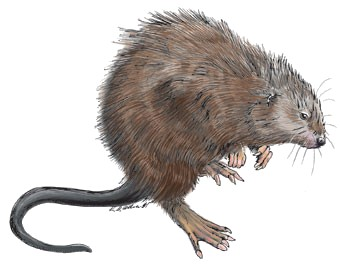
\includegraphics[width = 0.15\textwidth]{imgs/swmprat.png}} 
Don't forget to use your stickies: {\color{green} green} for done/ok, {\color{red} red} for problem
\end{frame}

%%%%%%
\begin{frame}[t]{Basic analyses with SWMPr}
\onslide<+->
How do we want to use the data? \\~\\
\onslide<+->
\begin{itemize}
\item What has happened at my site over time? \\~\\
\item Are there differences between sites? \\~\\
\item Can we remove seasonal trends? \\~\\
\item Are there differences between parameters? \\~\\
\item Others?
\end{itemize}
\end{frame}

%%%%%%
\begin{frame}[fragile]{Basic analyses with SWMPr 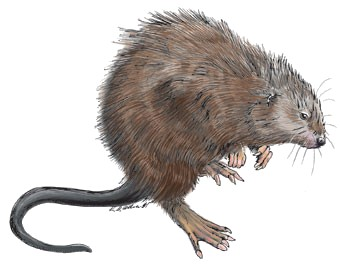
\includegraphics[width = 0.065\textwidth]{imgs/swmprat.png}}
\onslide<+->
Take a few minutes to acquaint yourself with the \Bigtxt{analyze} functions:
\begin{knitrout}\scriptsize
\definecolor{shadecolor}{rgb}{0.969, 0.969, 0.969}\color{fgcolor}\begin{kframe}
\begin{alltt}
\hlkwd{help.search}\hlstd{(}\hlstr{'analyze'}\hlstd{,} \hlkwc{package} \hlstd{=} \hlstr{'SWMPr'}\hlstd{)}
\end{alltt}
\end{kframe}
\end{knitrout}
\onslide<+->
Which functions simplify the data?  \\~\\
Which functions could you use to explore or visualize the data? \\~\\
Which functions are related to metabolism? 
\end{frame}

%%%%%%
\begin{frame}{Basic analyses with SWMPr - missing data}
Most datasets will have missing values - how do you deal with those? \\~\\
Remove? Set as mean? Replace with similar? \\~\\
SWMPr provides a function to interpolate missing data: \texttt{na.approx} \\~\\
To start, let's import and plot some data...
\end{frame}

%%%%%%
\begin{frame}[fragile]{Basic analyses with SWMPr - missing data 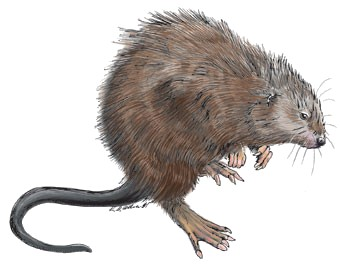
\includegraphics[width = 0.065\textwidth]{imgs/swmprat.png}}
\begin{itemize}
\item \onslide<1->
Import the 2012 water quality data for cbmmc from the `zip\_ex' folder (\texttt{?import\_local})
\onslide<2->
\begin{knitrout}\scriptsize
\definecolor{shadecolor}{rgb}{0.969, 0.969, 0.969}\color{fgcolor}\begin{kframe}
\begin{alltt}
\hlstd{mypath} \hlkwb{<-} \hlstr{'zip_ex'}
\hlstd{dat} \hlkwb{<-} \hlkwd{import_local}\hlstd{(mypath,} \hlstr{'cbmmcwq2012'}\hlstd{)}
\end{alltt}
\end{kframe}
\end{knitrout}
\vspace{0.1in}
\item \onslide<1->
Deal with QAQC columns (\texttt{?qaqc})
\onslide<3->
\begin{knitrout}\scriptsize
\definecolor{shadecolor}{rgb}{0.969, 0.969, 0.969}\color{fgcolor}\begin{kframe}
\begin{alltt}
\hlstd{tmp} \hlkwb{<-} \hlkwd{qaqc}\hlstd{(dat)}
\end{alltt}
\end{kframe}
\end{knitrout}
\vspace{0.1in}
\item \onslide<1->
Select two columns of interest (\texttt{?subset.swmpr})
\onslide<4->
\begin{knitrout}\scriptsize
\definecolor{shadecolor}{rgb}{0.969, 0.969, 0.969}\color{fgcolor}\begin{kframe}
\begin{alltt}
\hlstd{tmp} \hlkwb{<-} \hlkwd{subset}\hlstd{(tmp,} \hlkwc{select} \hlstd{=} \hlstr{'do_mgl'}\hlstd{,} \hlkwc{subset} \hlstd{=} \hlkwd{c}\hlstd{(}\hlstr{'2012-10-01 0:0'}\hlstd{,}
  \hlstr{'2012-10-31 0:0'}\hlstd{))}
\end{alltt}
\end{kframe}
\end{knitrout}
\vspace{0.1in}
\item \onslide<1->
Plot the data subset (\texttt{?plot.swmpr})
\onslide<5->
\begin{knitrout}\scriptsize
\definecolor{shadecolor}{rgb}{0.969, 0.969, 0.969}\color{fgcolor}\begin{kframe}
\begin{alltt}
\hlkwd{plot}\hlstd{(tmp)}
\end{alltt}
\end{kframe}
\end{knitrout}
\end{itemize}
\end{frame}

%%%%%%
\begin{frame}[fragile]{Basic analyses with SWMPr - missing data}
\begin{knitrout}\scriptsize
\definecolor{shadecolor}{rgb}{0.969, 0.969, 0.969}\color{fgcolor}

{\centering 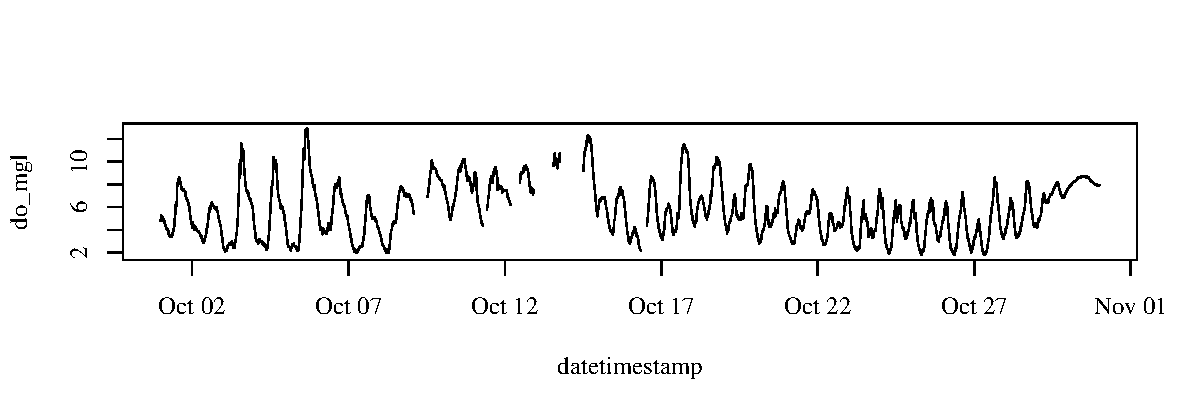
\includegraphics[width=0.9\textwidth]{figure/unnamed-chunk-6-1} 

}



\end{knitrout}
Notice the missing data around October 12\textsuperscript{th} \\~\\
The \texttt{na.approx} function (\texttt{?na.approx.swmpr}) has three arguments:
\begin{itemize}
\item \texttt{object}: swmpr data object to fill
\item \texttt{params}: name(s) of parameter to fill
\item \texttt{maxgap}: maximum gap size to interpolate
\end{itemize}
\end{frame}

%%%%%%
\begin{frame}[fragile]{Basic analyses with SWMPr - missing data 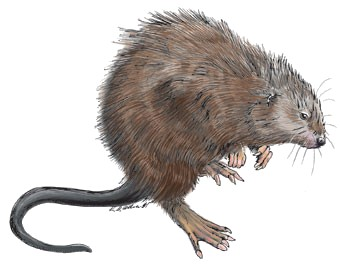
\includegraphics[width = 0.065\textwidth]{imgs/swmprat.png}}
\begin{itemize}
\item \onslide<1->
Use \texttt{na.approx} to interpolate the missing data (\texttt{?na.approx.swmpr})
\onslide<2->
\begin{knitrout}\scriptsize
\definecolor{shadecolor}{rgb}{0.969, 0.969, 0.969}\color{fgcolor}\begin{kframe}
\begin{alltt}
\hlstd{tmp2} \hlkwb{<-} \hlkwd{na.approx}\hlstd{(tmp,} \hlkwc{params} \hlstd{=} \hlstr{'do_mgl'}\hlstd{,} \hlkwc{maxgap} \hlstd{=} \hlnum{100}\hlstd{)}
\end{alltt}
\end{kframe}
\end{knitrout}
\vspace{0.1in}
\item \onslide<1->
Plot the two to see the differences (\texttt{?plot.swmpr})
\onslide<3->
\begin{knitrout}\scriptsize
\definecolor{shadecolor}{rgb}{0.969, 0.969, 0.969}\color{fgcolor}\begin{kframe}
\begin{alltt}
\hlkwd{plot}\hlstd{(tmp)}
\hlkwd{plot}\hlstd{(tmp2)}
\end{alltt}
\end{kframe}
\end{knitrout}
\end{itemize}
\onslide<3->
\vspace{-0.4in}
\begin{knitrout}\scriptsize
\definecolor{shadecolor}{rgb}{0.969, 0.969, 0.969}\color{fgcolor}

{\centering 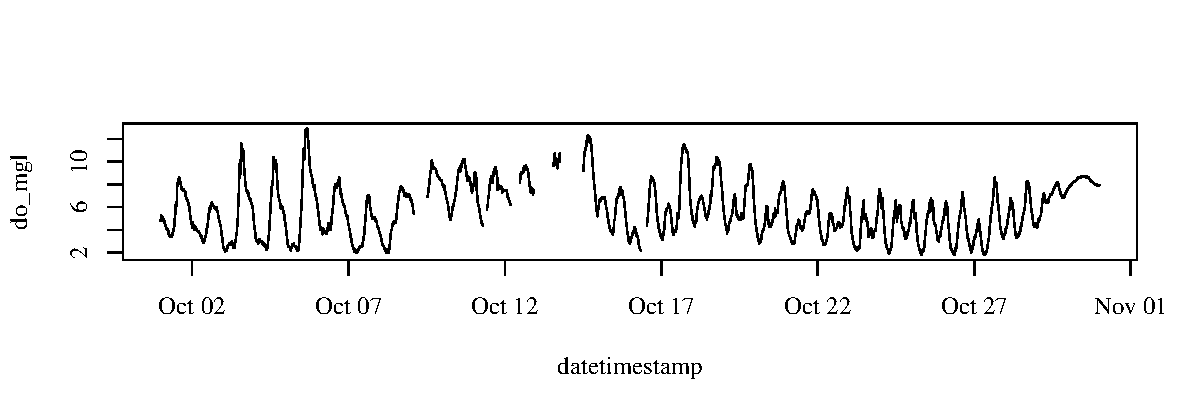
\includegraphics[width=0.9\textwidth]{figure/unnamed-chunk-9-1} 

}



\end{knitrout}
\vspace{-0.5in}
\begin{knitrout}\scriptsize
\definecolor{shadecolor}{rgb}{0.969, 0.969, 0.969}\color{fgcolor}

{\centering 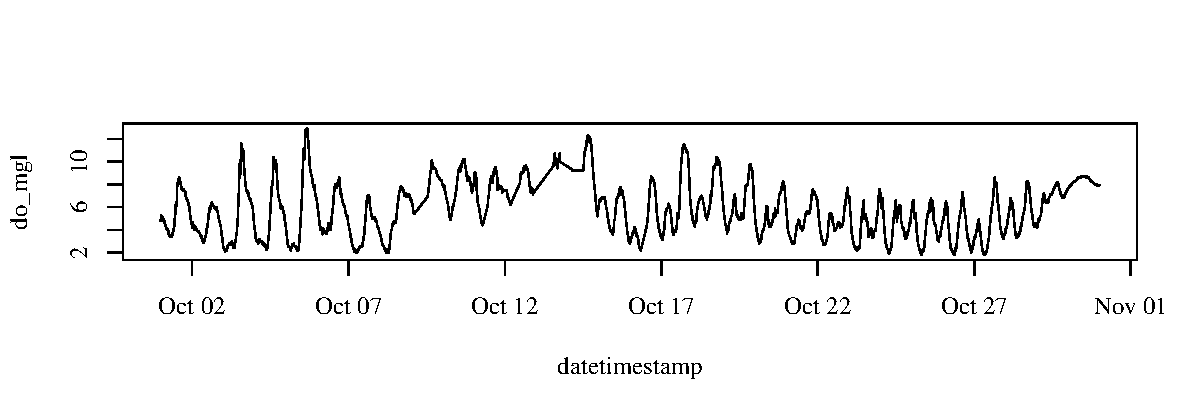
\includegraphics[width=0.9\textwidth]{figure/unnamed-chunk-10-1} 

}



\end{knitrout}
\end{frame}

%%%%%%
\begin{frame}[fragile]{Basic analyses with SWMPr - smoothing data}
Now we know how to fill missing data, let's see how it can help...\\~\\
Trend evaluation often considers variation at different spatial scales \\~\\
As an example, we want to evaluate variation in dissolved oxygen at seasonal or annual scales \\~\\
\begin{knitrout}\scriptsize
\definecolor{shadecolor}{rgb}{0.969, 0.969, 0.969}\color{fgcolor}

{\centering 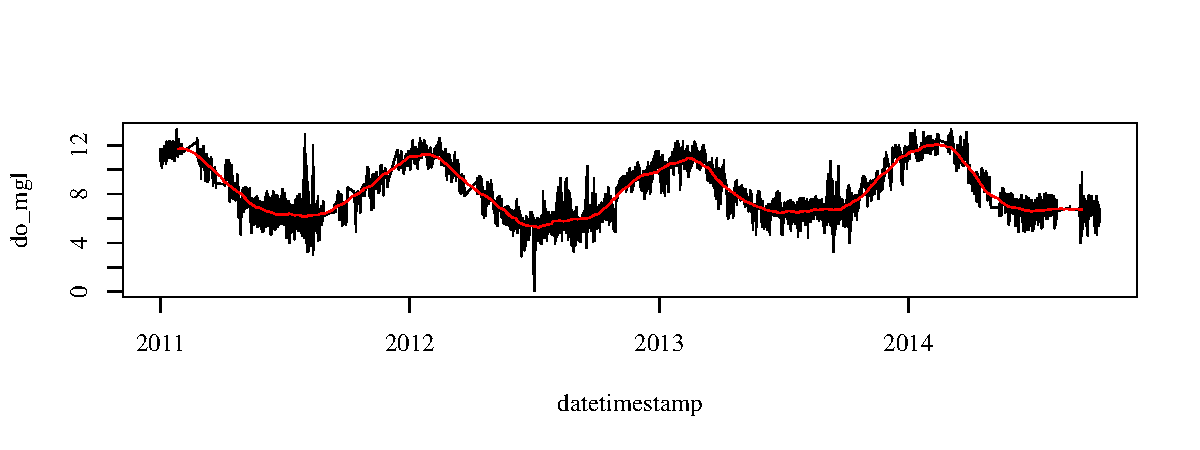
\includegraphics[width=\textwidth]{figure/unnamed-chunk-11-1} 

}



\end{knitrout}
\end{frame}

%%%%%%
\begin{frame}[containsverbatim]{Analysis 2 - Smoothing and aggregation}
The \texttt{smoother} function (\texttt{?smoother}) calculates a moving window average of a time series \\~\\
\begin{itemize}
\item \texttt{x}: Input data object \\~\\
\item \texttt{window}: the size of the smoothing window, defaults to five observations at the current time step \\~\\
\item \texttt{sides}: what defines the window, centered on an observation (2, default) or use only the preceding observations (1)  \\~\\
\item \texttt{params}: which parameters to smooth, default all \\~\\
\end{itemize}
What would be a good window to look at seasonal or annual variation?
\end{frame}

%%%%%%
\begin{frame}[fragile]{Basic analyses with SWMPr - smoothing data 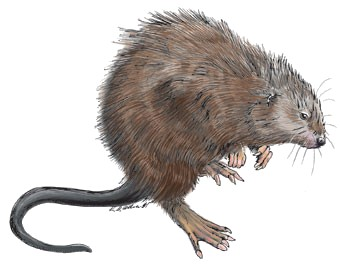
\includegraphics[width = 0.065\textwidth]{imgs/swmprat.png}}
\begin{itemize}
\item \onslide<1->
Import all years of water quality data for cbmip from the `zip\_ex' folder
\onslide<2->
\begin{knitrout}\scriptsize
\definecolor{shadecolor}{rgb}{0.969, 0.969, 0.969}\color{fgcolor}\begin{kframe}
\begin{alltt}
\hlstd{mypath} \hlkwb{<-} \hlstr{'zip_ex'}
\hlstd{dat} \hlkwb{<-} \hlkwd{import_local}\hlstd{(mypath,} \hlstr{'cbmipwq'}\hlstd{)}
\end{alltt}
\end{kframe}
\end{knitrout}
\vspace{0.1in}
\item \onslide<1->
Deal with QAQC columns and subset DO
\onslide<3->
\begin{knitrout}\scriptsize
\definecolor{shadecolor}{rgb}{0.969, 0.969, 0.969}\color{fgcolor}\begin{kframe}
\begin{alltt}
\hlstd{tmp} \hlkwb{<-} \hlkwd{qaqc}\hlstd{(dat)}
\hlstd{tmp} \hlkwb{<-} \hlkwd{subset}\hlstd{(dat,} \hlkwc{select} \hlstd{=} \hlstr{'do_mgl'}\hlstd{)}
\end{alltt}
\end{kframe}
\end{knitrout}
\vspace{0.1in}
\item \onslide<1->
Use \texttt{smoother} to remove daily and short-term variation, which window to use?
\onslide<4->
\begin{knitrout}\scriptsize
\definecolor{shadecolor}{rgb}{0.969, 0.969, 0.969}\color{fgcolor}\begin{kframe}
\begin{alltt}
\hlstd{do_smooth} \hlkwb{<-} \hlkwd{smoother}\hlstd{(tmp2,} \hlkwc{window} \hlstd{=} \hlnum{5000}\hlstd{)}
\end{alltt}
\end{kframe}
\end{knitrout}
\vspace{0.1in}
\item \onslide<1->
Plot results (see \texttt{?plot.swmpr} and \texttt{?lines.swmpr})
\onslide<5->
\begin{knitrout}\scriptsize
\definecolor{shadecolor}{rgb}{0.969, 0.969, 0.969}\color{fgcolor}\begin{kframe}
\begin{alltt}
\hlkwd{plot}\hlstd{(tmp)}
\hlkwd{lines}\hlstd{(do_smooth,} \hlkwc{col} \hlstd{=} \hlstr{'red'}\hlstd{)}
\end{alltt}
\end{kframe}
\end{knitrout}
\end{itemize}
\end{frame}

%%%%%%
\begin{frame}[fragile]{Basic analyses with SWMPr - smoothing data}
\begin{knitrout}\scriptsize
\definecolor{shadecolor}{rgb}{0.969, 0.969, 0.969}\color{fgcolor}

{\centering 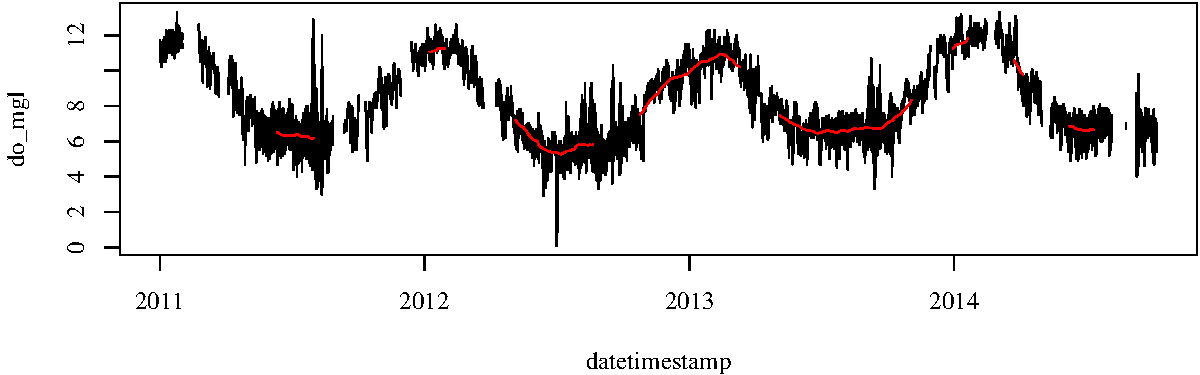
\includegraphics[width=0.9\textwidth]{figure/unnamed-chunk-16-1} 

}



\end{knitrout}
What happened?  \\~\\
How can we fix the problem? 
\end{frame}

%%%%%%
\begin{frame}[fragile,t]{Basic analyses with SWMPr - smoothing data 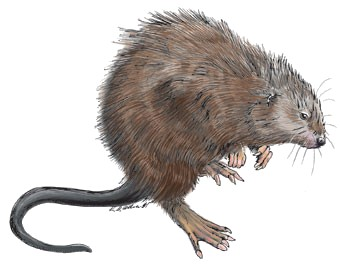
\includegraphics[width = 0.065\textwidth]{imgs/swmprat.png}}
\onslide<+->
Repeat the analysis but use \texttt{na.approx} to fill missing data
\begin{knitrout}\scriptsize
\definecolor{shadecolor}{rgb}{0.969, 0.969, 0.969}\color{fgcolor}\begin{kframe}
\begin{alltt}
\hlstd{mypath} \hlkwb{<-} \hlstr{'zip_ex'}
\hlstd{dat} \hlkwb{<-} \hlkwd{import_local}\hlstd{(mypath,} \hlstr{'cbmipwq'}\hlstd{)}
\hlstd{tmp} \hlkwb{<-} \hlkwd{qaqc}\hlstd{(dat)}
\hlstd{tmp} \hlkwb{<-} \hlkwd{subset}\hlstd{(tmp,} \hlkwc{select} \hlstd{=} \hlstr{'do_mgl'}\hlstd{)}
\hlstd{do_smooth} \hlkwb{<-} \hlkwd{smoother}\hlstd{(tmp,} \hlkwc{window} \hlstd{=} \hlnum{5000}\hlstd{)}
\hlkwd{plot}\hlstd{(tmp)}
\hlkwd{lines}\hlstd{(do_smooth,} \hlkwc{col} \hlstd{=} \hlstr{'red'}\hlstd{)}
\end{alltt}
\end{kframe}
\end{knitrout}
Where would you use \texttt{na.approx}?
\onslide<+->
\begin{knitrout}\scriptsize
\definecolor{shadecolor}{rgb}{0.969, 0.969, 0.969}\color{fgcolor}\begin{kframe}
\begin{alltt}
\hlstd{mypath} \hlkwb{<-} \hlstr{'zip_ex'}
\hlstd{dat} \hlkwb{<-} \hlkwd{import_local}\hlstd{(mypath,} \hlstr{'cbmipwq'}\hlstd{)}
\hlstd{tmp} \hlkwb{<-} \hlkwd{qaqc}\hlstd{(dat)}
\hlstd{tmp} \hlkwb{<-} \hlkwd{subset}\hlstd{(tmp,} \hlkwc{select} \hlstd{=} \hlstr{'do_mgl'}\hlstd{)}
\hlstd{tmp} \hlkwb{<-} \hlkwd{na.approx}\hlstd{(tmp,} \hlkwc{maxgap} \hlstd{=} \hlnum{5000}\hlstd{)}
\hlstd{do_smooth} \hlkwb{<-} \hlkwd{smoother}\hlstd{(tmp,} \hlkwc{window} \hlstd{=} \hlnum{5000}\hlstd{)}
\hlkwd{plot}\hlstd{(tmp)}
\hlkwd{lines}\hlstd{(do_smooth,} \hlkwc{col} \hlstd{=} \hlstr{'red'}\hlstd{)}
\end{alltt}
\end{kframe}
\end{knitrout}
\onslide<+->
Bonus: Try changing \texttt{maxgap} or \texttt{window}
\end{frame}

%%%%%%
\begin{frame}[containsverbatim]{Basic analyses with SWMPr - aggregating data}
Finally, we can use \texttt{aggreswmp} to summarize and plot for an alternative interpretation \\~\\
\texttt{aggreswmp} has five main arguments: \\~\\
\begin{itemize}
\item \texttt{swmpr\_in}: input data object \\~\\
\item \texttt{by}: aggregation period (`years', `quarters', etc.) \\~\\
\item \texttt{FUN}: aggregation function, defaults to mean \\~\\
\item \texttt{params}: which parameters to aggregate, defaults all \\~\\
\item \texttt{aggs\_out}: get the raw data, use this to make plots
\end{itemize}
\end{frame}

%%%%%%
\begin{frame}[fragile,t]{Basic analyses with SWMPr - aggregating data 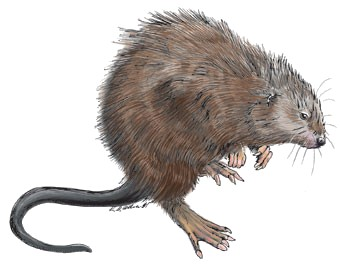
\includegraphics[width = 0.065\textwidth]{imgs/swmprat.png}}
\begin{itemize}
\item \onslide<1->
Import all years of water quality data for cbmip from the `zip\_ex' folder, QAQC cleanup, and subset DO
\onslide<2->
\begin{knitrout}\scriptsize
\definecolor{shadecolor}{rgb}{0.969, 0.969, 0.969}\color{fgcolor}\begin{kframe}
\begin{alltt}
\hlstd{mypath} \hlkwb{<-} \hlstr{'zip_ex'}
\hlstd{dat} \hlkwb{<-} \hlkwd{import_local}\hlstd{(mypath,} \hlstr{'cbmipwq'}\hlstd{)}
\hlstd{tmp} \hlkwb{<-} \hlkwd{qaqc}\hlstd{(dat)}
\hlstd{tmp} \hlkwb{<-} \hlkwd{subset}\hlstd{(tmp,} \hlkwc{select} \hlstd{=} \hlstr{'do_mgl'}\hlstd{)}
\end{alltt}
\end{kframe}
\end{knitrout}
\vspace{0.1in}
\item \onslide<1->
Use \texttt{aggreswmp} (\texttt{?aggreswmp}) to get quarterly summaries of the data
\onslide<3->
\begin{knitrout}\scriptsize
\definecolor{shadecolor}{rgb}{0.969, 0.969, 0.969}\color{fgcolor}\begin{kframe}
\begin{alltt}
\hlstd{aggtmp} \hlkwb{<-} \hlkwd{aggreswmp}\hlstd{(tmp,} \hlkwc{by} \hlstd{=} \hlstr{'quarters'}\hlstd{)}
\end{alltt}
\end{kframe}
\end{knitrout}
\vspace{0.1in}
\item \onslide<4->
Bonus: Try different aggregation periods
\onslide<5->
\begin{knitrout}\scriptsize
\definecolor{shadecolor}{rgb}{0.969, 0.969, 0.969}\color{fgcolor}\begin{kframe}
\begin{alltt}
\hlstd{aggtmp} \hlkwb{<-} \hlkwd{aggreswmp}\hlstd{(tmp,} \hlkwc{by} \hlstd{=} \hlstr{'years'}\hlstd{)}
\hlstd{aggtmp} \hlkwb{<-} \hlkwd{aggreswmp}\hlstd{(tmp,} \hlkwc{by} \hlstd{=} \hlstr{'weeks'}\hlstd{)}
\end{alltt}
\end{kframe}
\end{knitrout}
\vspace{0.1in}
\item
\onslide<4->
Bonus: Try different aggregation functions
\onslide<6->
\begin{knitrout}\scriptsize
\definecolor{shadecolor}{rgb}{0.969, 0.969, 0.969}\color{fgcolor}\begin{kframe}
\begin{alltt}
\hlstd{fun_in} \hlkwb{<-} \hlkwa{function}\hlstd{(}\hlkwc{x}\hlstd{)}  \hlkwd{var}\hlstd{(x,} \hlkwc{na.rm} \hlstd{=} \hlnum{TRUE}\hlstd{)}
\hlstd{aggtmp} \hlkwb{<-} \hlkwd{aggreswmp}\hlstd{(tmp,} \hlkwc{FUN} \hlstd{= fun_in,} \hlstr{'years'}\hlstd{)}
\end{alltt}
\end{kframe}
\end{knitrout}
\vspace{0.1in}
\end{itemize}
\end{frame}

%%%%%%
\begin{frame}[fragile]{Basic analyses with SWMPr - aggregating data 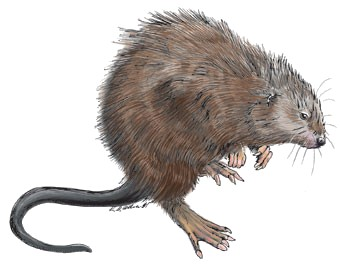
\includegraphics[width = 0.065\textwidth]{imgs/swmprat.png}}
\onslide<+->
Plot the aggregated data by quarters - use \texttt{aggs\_out = TRUE}
\onslide<+->
\begin{knitrout}\scriptsize
\definecolor{shadecolor}{rgb}{0.969, 0.969, 0.969}\color{fgcolor}\begin{kframe}
\begin{alltt}
\hlcom{# use aggs_out to get all}
\hlstd{aggtmp} \hlkwb{<-} \hlkwd{aggreswmp}\hlstd{(tmp,} \hlkwc{by} \hlstd{=} \hlstr{'quarters'}\hlstd{,} \hlkwc{aggs_out} \hlstd{=} \hlnum{TRUE}\hlstd{)}
\end{alltt}
\end{kframe}
\end{knitrout}
\onslide<+->
Then use \texttt{boxplot} (\texttt{?boxplot}) from the R stats package
\onslide<+->
\begin{knitrout}\scriptsize
\definecolor{shadecolor}{rgb}{0.969, 0.969, 0.969}\color{fgcolor}\begin{kframe}
\begin{alltt}
\hlcom{# use boxplot }
\hlkwd{boxplot}\hlstd{(do_mgl} \hlopt{~} \hlstd{datetimestamp,} \hlkwc{data} \hlstd{= aggtmp,} \hlkwc{ylab} \hlstd{=} \hlstr{'do_mgl'}\hlstd{,} \hlkwc{ylim} \hlstd{=} \hlkwd{c}\hlstd{(}\hlnum{0}\hlstd{,} \hlnum{15}\hlstd{))}
\end{alltt}
\end{kframe}

{\centering 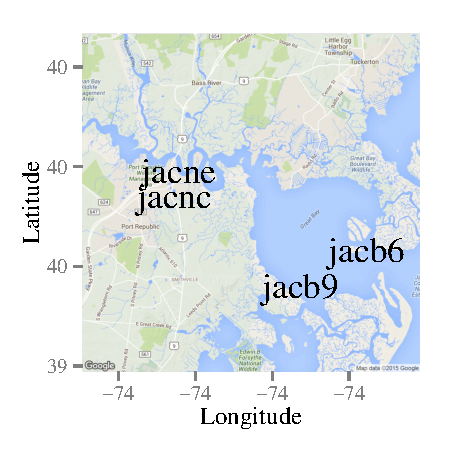
\includegraphics[width=0.9\textwidth]{figure/unnamed-chunk-24-1} 

}



\end{knitrout}
\onslide<+->
\vspace{-0.2in}
Have a look at the data from \texttt{aggs_out = TRUE} and \texttt{aggs_out = FALSE}, how do they differ and why?
\end{frame}

%%%%%%
\begin{frame}[fragile]{Plotting functions in SWMPr}
R provides near limitless options to visualize data - a full coverage of these tools would take days \\~\\
We will briefly go over some key plotting functions in SWMPr, each is designed for simplicity and efficiency to summarize lots of data \\~\\
Plotting functions in SWMPr: \\~\\
\begin{itemize}
\item \texttt{decomp}: time series decomposition
\item \texttt{decomp\_cj}: time series decomposition, alternative
\item \texttt{map\_reserve}: plot a basic map of a reserve
\item \texttt{overplot}: plot multiple parameters on the same plot
\item \texttt{plot\_metab}: plot metabolism estimates
\item \texttt{plot\_summary}: plot multiple summaries for a parameter
\end{itemize}
\end{frame}

%%%%%%
\begin{frame}[fragile, t]{Plotting functions in SWMPr 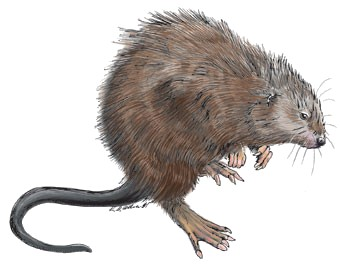
\includegraphics[width = 0.065\textwidth]{imgs/swmprat.png}}
\onslide<+->
The \texttt{map\_reserve} function can be used to map sites:
\begin{itemize}
\item \texttt{nerr\_site\_id}: site(s) to map, usually first three letters
\item \texttt{zoom}: zoom factor for the map (usually between 5--15)
\item \texttt{map\_type}: \texttt{`terrain'}, \texttt{`satellite'}, \texttt{`roadmap'}, or \texttt{`hybrid'}
\end{itemize}
\begin{columns}[T]
\begin{column}{0.45\textwidth}
\begin{knitrout}\scriptsize
\definecolor{shadecolor}{rgb}{0.969, 0.969, 0.969}\color{fgcolor}\begin{kframe}
\begin{alltt}
\hlcom{# try any of these examples}
\hlkwd{map_reserve}\hlstd{(}\hlstr{'jac'}\hlstd{)}

\hlkwd{map_reserve}\hlstd{(}\hlstr{'elk'}\hlstd{,} \hlkwc{zoom} \hlstd{=} \hlnum{13}\hlstd{,}
  \hlkwc{map_type} \hlstd{=} \hlstr{'hybrid'}\hlstd{)}

\hlkwd{map_reserve}\hlstd{(}\hlstr{'gtmss'}\hlstd{,} \hlkwc{zoom} \hlstd{=} \hlnum{15}\hlstd{,}
  \hlkwc{map_type} \hlstd{=} \hlstr{'satellite'}\hlstd{,}
  \hlkwc{text_col} \hlstd{=} \hlstr{'lightblue'}\hlstd{)}
\end{alltt}
\end{kframe}
\end{knitrout}
\end{column}
\begin{column}{0.45\textwidth}
\onslide<+->
\begin{knitrout}\scriptsize
\definecolor{shadecolor}{rgb}{0.969, 0.969, 0.969}\color{fgcolor}

{\centering 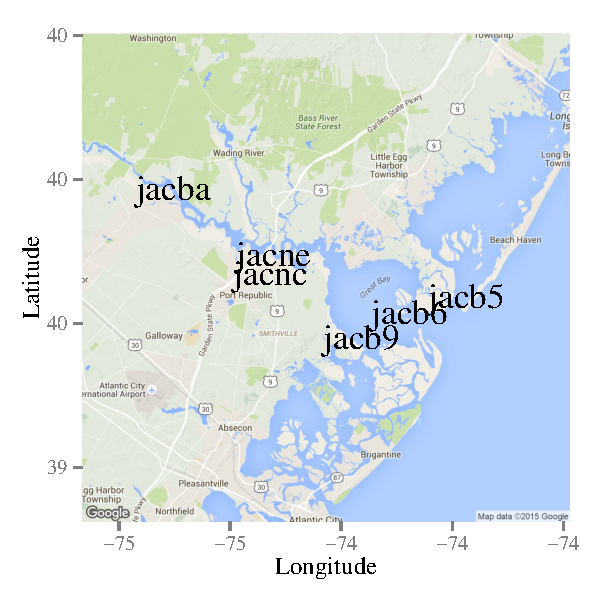
\includegraphics[width=\textwidth]{figure/unnamed-chunk-26-1} 

}



\end{knitrout}
\end{column}
\end{columns}
\end{frame}

%%%%%%
\begin{frame}[fragile, t]{Plotting functions in SWMPr 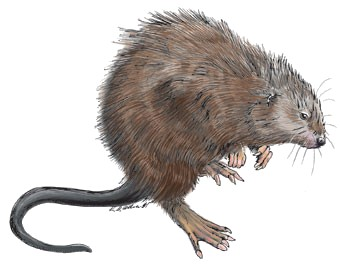
\includegraphics[width = 0.065\textwidth]{imgs/swmprat.png}}
\onslide<1->
The \texttt{overplot} function can be used to plot one to many time series:\\~\\
\begin{itemize}
\item \texttt{dat_in}: input \texttt{swmpr} object
\item \texttt{select}: parameter(s) to plot (passed to \texttt{subset})
\item \texttt{subset}: date ranges to plot (passed to \texttt{subset})\\~\\
\end{itemize}
\onslide<2->
Import the 2011 data for cbmip
\onslide<3->
\begin{knitrout}\scriptsize
\definecolor{shadecolor}{rgb}{0.969, 0.969, 0.969}\color{fgcolor}\begin{kframe}
\begin{alltt}
\hlcom{# import}
\hlstd{mypath} \hlkwb{<-} \hlstr{'zip_ex'}
\hlstd{dat} \hlkwb{<-} \hlkwd{import_local}\hlstd{(mypath,} \hlstr{'cbmipwq2011'}\hlstd{)}
\end{alltt}
\end{kframe}
\end{knitrout}
\onslide<2->
Plot DO, temperature, and salinity for August (\texttt{?overplot})
\onslide<4->
\begin{knitrout}\scriptsize
\definecolor{shadecolor}{rgb}{0.969, 0.969, 0.969}\color{fgcolor}\begin{kframe}
\begin{alltt}
\hlcom{# plot}
\hlkwd{overplot}\hlstd{(dat,} \hlkwc{select} \hlstd{=} \hlkwd{c}\hlstd{(}\hlstr{'do_mgl'}\hlstd{,} \hlstr{'temp'}\hlstd{),}
  \hlkwc{subset} \hlstd{=} \hlkwd{c}\hlstd{(}\hlstr{'2011-08-01 0:0'}\hlstd{,} \hlstr{'2011-08-31 0:0'}\hlstd{))}
\end{alltt}
\end{kframe}
\end{knitrout}
\end{frame}

%%%%%% 
\begin{frame}[fragile, t]{Plotting functions in SWMPr}
\begin{knitrout}\scriptsize
\definecolor{shadecolor}{rgb}{0.969, 0.969, 0.969}\color{fgcolor}\begin{kframe}
\begin{alltt}
\hlcom{# plot}
\hlkwd{overplot}\hlstd{(dat,} \hlkwc{select} \hlstd{=} \hlkwd{c}\hlstd{(}\hlstr{'do_mgl'}\hlstd{,} \hlstr{'temp'}\hlstd{),}
  \hlkwc{subset} \hlstd{=} \hlkwd{c}\hlstd{(}\hlstr{'2011-08-01 0:0'}\hlstd{,} \hlstr{'2011-08-31 0:0'}\hlstd{))}
\end{alltt}
\end{kframe}

{\centering 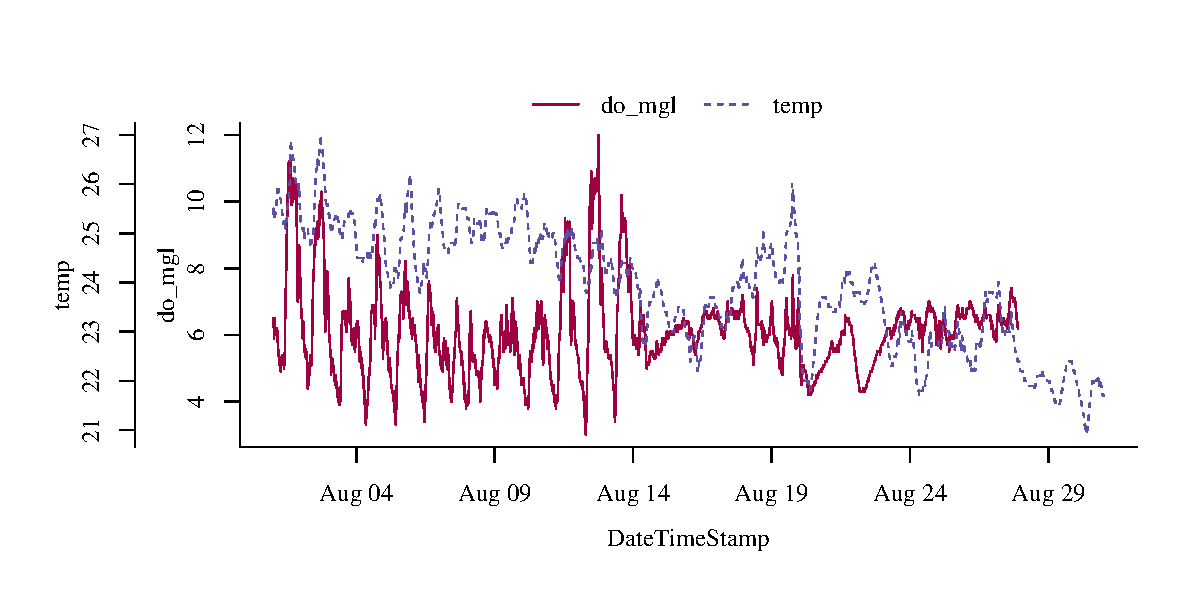
\includegraphics[width=\textwidth]{figure/unnamed-chunk-29-1} 

}



\end{knitrout}
\end{frame}

%%%%%%
\begin{frame}[fragile, t]{Plotting functions in SWMPr 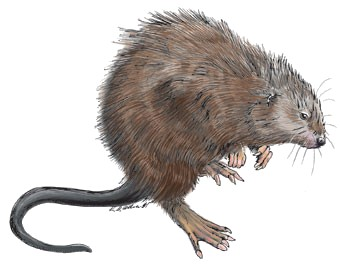
\includegraphics[width = 0.065\textwidth]{imgs/swmprat.png}}
\onslide<1->
The \texttt{plot_summary} function can be used to summarize a parameter across the time series\\~\\
\begin{itemize}
\item \texttt{swmpr\_in}: input swmpr object
\item \texttt{param}: parameter to summarize
\item \texttt{years}: years to plot\\~\\
\end{itemize}
\onslide<1->
Import all years of data for cbmip, plot a summary of temperature (\texttt{?plot\_summary})
\onslide<2->
\begin{knitrout}\scriptsize
\definecolor{shadecolor}{rgb}{0.969, 0.969, 0.969}\color{fgcolor}\begin{kframe}
\begin{alltt}
\hlcom{# import}
\hlstd{mypath} \hlkwb{<-} \hlstr{'zip_ex'}
\hlstd{dat} \hlkwb{<-} \hlkwd{import_local}\hlstd{(mypath,} \hlstr{'cbmipwq'}\hlstd{)}

\hlcom{# plot}
\hlkwd{plot_summary}\hlstd{(dat,} \hlstr{'temp'}\hlstd{)}
\end{alltt}
\end{kframe}
\end{knitrout}
\end{frame}

%%%%%%
\begin{frame}[fragile, t]{Plotting functions in SWMPr}

\begin{knitrout}\scriptsize
\definecolor{shadecolor}{rgb}{0.969, 0.969, 0.969}\color{fgcolor}\begin{kframe}
\begin{alltt}
\hlcom{# plot}
\hlkwd{plot_summary}\hlstd{(dat,} \hlstr{'temp'}\hlstd{)}
\end{alltt}
\end{kframe}

{\centering 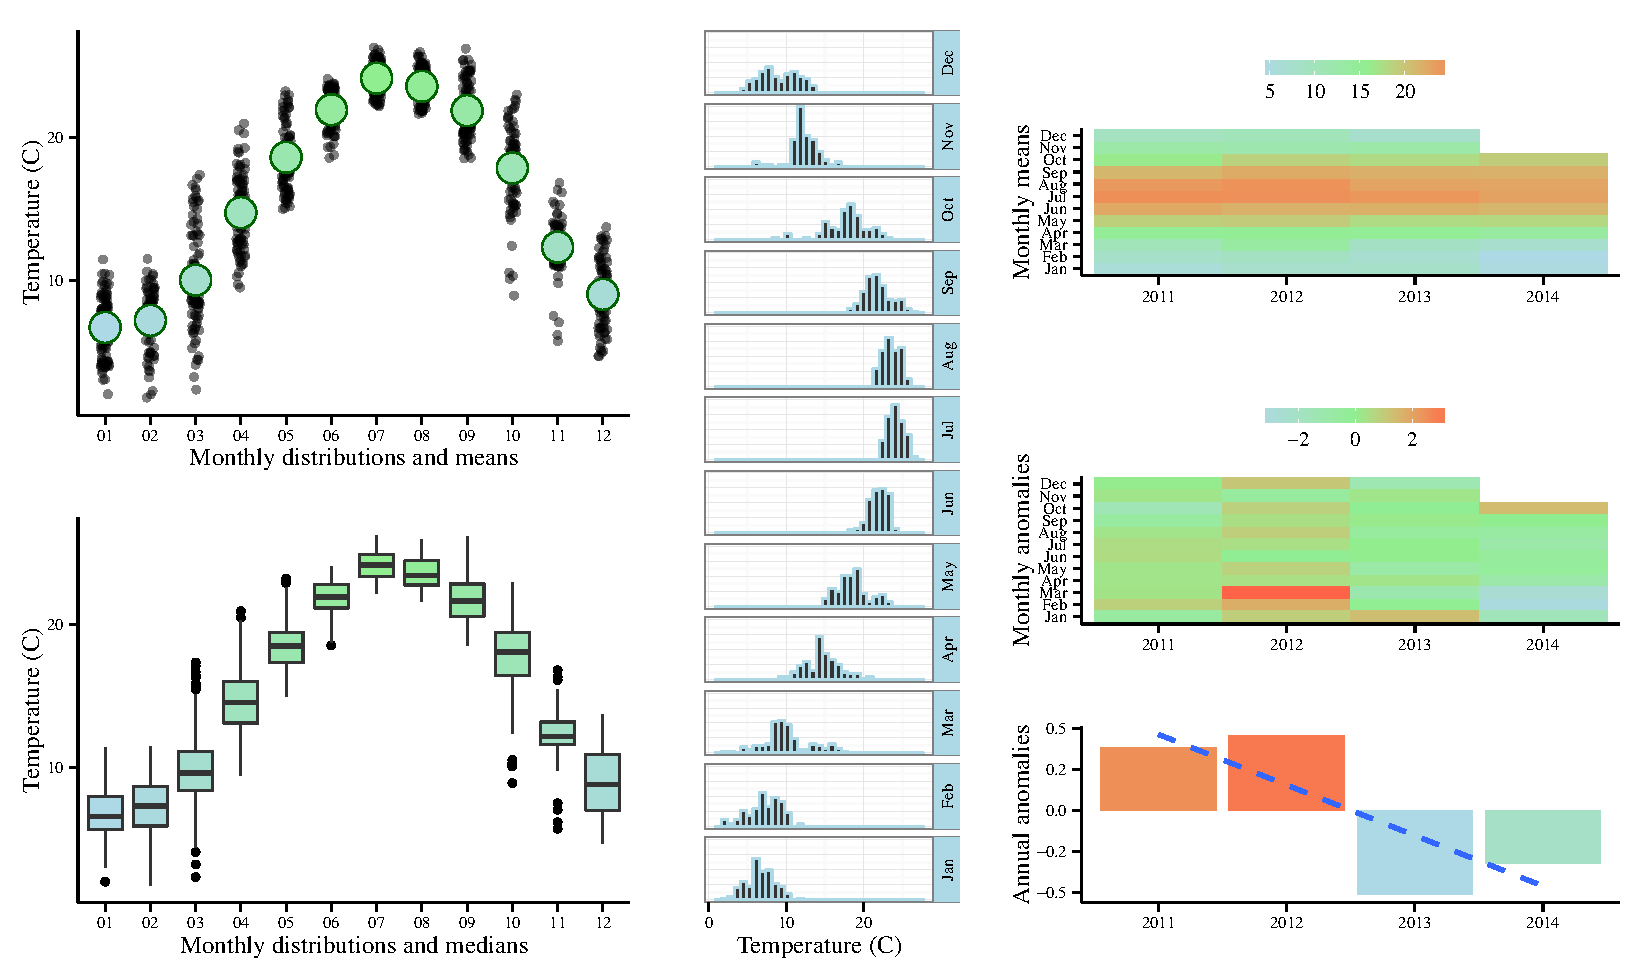
\includegraphics[width=0.9\textwidth]{figure/unnamed-chunk-32-1} 

}



\end{knitrout}
\end{frame}

%%%%%%
\begin{frame}{Additional resources}
You've been exposed to some basic tools to \Bigtxt{retrieve}, \Bigtxt{organize}, and \Bigtxt{analyze} SWMP data with SWMPr \\~\\
There are multiple resources available for continued learning: \\~\\
\begin{itemize}
\item \href{http://swmprats.net/}{swmprats.net}
\begin{itemize}
\item User forum to post questions, plot of the month
\item Widgets for data viz
\item Access to workshop materials
\item Access to 2014 workshop materials \\~\\
\end{itemize}
\item SWMPr online reference \href{https://cran.r-project.org/web/packages/SWMPr/SWMPr.pdf}{manual}: list of all functions \\~\\
\item SWMPr \href{https://github.com/fawda123/swmp_workshop_2015/raw/master/cookbook/swmpr_cookbook.pdf}{cookbook}: step-by-step scripts as stand-alone analyses \\~\\
\item Email instructors: \href{mailto:beck.marcus@epa.gov}{beck.marcus@epa.gov}, \href{todd.obrien@noaa.gov}{todd.obrien@noaa.gov}
\end{itemize}
\end{frame}

%%%%%%
\begin{frame}
\vspace{0.3in}
\centerline{
\begin{tikzpicture}
  \node[drop shadow={shadow xshift=0ex,shadow yshift=0ex},fill=white,draw] at (0,0) {
\includegraphics[width=0.9\textwidth]{imgs/workshop_logo.png}};
\end{tikzpicture}}
\vspace{0.5in}
\Large
\centerline{\Bigtxt{Questions??}}
\end{frame}

\end{document}
